% ==========================================================================
% Simulations section — Monte Carlo evidence on joint vs two-step estimation
% Generated from the production sweep of 2026-08-22 (6,900 replications).
% Fragments: tables/sim_point.tex, tables/sim_coverage.tex,
%            tables/sim_vi_appendix.tex; figures/sim_{distributions,bias,
%            coverage,mechanism}.pdf.  Cite key for Battaglia--Christensen--
%            Hansen--Sacher (2025): \citet{BattagliaEtAl2025}.
% ==========================================================================

\section{Monte Carlo evidence}
\label{sec:simulations}

This section evaluates the finite-sample behavior of the amortized joint
estimator in a setting where the econometric theory of regression on
estimated latent factors makes sharp predictions.
\citet{BattagliaEtAl2025} show that the two-step strategy---estimate latent
factors from unstructured data, then regress an outcome on the
estimates---carries a first-order asymptotic bias whenever measurement error
per observation does not vanish relative to sampling error (their
$\kappa>0$ regime), and that the bias takes the form of a location shift:
the two-step sampling distribution has essentially the correct spread but
the wrong center.  Their proposed remedy is joint likelihood estimation of
the measurement model and the regression.  We implement exactly that remedy
with amortized variational inference and ask three questions.  (i)~Is the
joint estimator consistent, with the parametric $\sqrt{n}$ rate and a
Gaussian sampling distribution?  (ii)~How badly does two-step inference fail
in the $\kappa>0$ regime, and does the failure match the theory
quantitatively?  (iii)~Can a practitioner obtain valid confidence intervals
from the joint fit with off-the-shelf tools?  The answers are yes, exactly
as predicted, and yes---via a post-fit least-squares readout with a one-line
standard-error correction.

\subsection{Design}
\label{sec:sim-design}

\paragraph{Data-generating process.}
Each observation $i=1,\dots,n$ has a binary covariate
$x_i\sim\mathrm{Bernoulli}(1/2)$ (a ``party label''), a scalar latent
factor (``ideal point'')
\begin{equation}
  \theta_i \;=\; \beta_0 + \beta_1 x_i + u_i,
  \qquad u_i\sim N(0,\sigma_u^2),
  \label{eq:sim-structural}
\end{equation}
and an outcome
\begin{equation}
  y_i \;=\; c\,\theta_i + \varepsilon_i,
  \qquad \varepsilon_i\sim N(0,\sigma_\varepsilon^2).
  \label{eq:sim-outcome}
\end{equation}
We set $\beta_0=0$, $\beta_1=1$, $\sigma_u=1$, $c=1$,
$\sigma_\varepsilon=1$, so the marginal standard deviation of the factor is
$\sigma_\theta=\sqrt{1.25}\approx1.118$.  The factor is measured through
one of two channels, holding the number of items $J$ fixed as $n$ grows:

\begin{itemize}
\item \emph{Roll-call votes (2PL IRT).}  Binary responses
  $V_{ij}\sim\mathrm{Bernoulli}\!\left(\Lambda(b_j\theta_i-d_j)\right)$,
  $j=1,\dots,J$, with $\Lambda$ the logistic cdf, discriminations
  $b_j\sim N(0,1)$ and difficulties $d_j\sim N(0,0.5)$.  This is the
  workhorse ideal-point measurement model and a nonlinear likelihood for
  which the exact posterior is not available in closed form.
\item \emph{Linear--Gaussian (validation rung).}  Continuous features
  $w_{ij}=\lambda_j\theta_i+\delta_j+\nu_{ij}$,
  $\nu_{ij}\sim N(0,\sigma_w^2)$ with $\sigma_w^2$ known, loadings
  $\lambda_j\sim N(0,0.25^2)$ and intercepts $\delta_j\sim N(0,0.5)$.  Here
  the exact posterior of $\theta_i$ is Gaussian and lies inside the
  variational family, so the ELBO maximizer coincides with the exact
  marginal maximum-likelihood estimator: any failure on this rung would
  indicate an optimization problem rather than a limitation of variational
  inference.  The loading scale is chosen so that the measurement design has
  the same reliability ($\approx0.85$) as the $J=25$ vote design.
\end{itemize}

The item parameters $(b_j,d_j)$ and $(\lambda_j,\delta_j)$ are drawn once
and held fixed across all replications and all sample sizes (a fixed
measurement design, the frame in which classical repeated-sampling
statements---and those of \citealp{BattagliaEtAl2025}---are made).  Each
replication redraws $(x_i,u_i,\varepsilon_i)$ and the measurement noise.
The core design crosses the two channels with
$n\in\{1{,}000,\,4{,}000,\,16{,}000\}$ at $J=25$, with $1{,}000$
replications per cell.  A reliability grid adds
$J\in\{10,50,100\}$ at $n=4{,}000$ in the vote channel ($300$ replications
per cell).  Fixing $J$ while $n$ grows is the starkest version of the
$\kappa>0$ regime: per-unit measurement error is $O(1/J)$ and does not
shrink, while sampling error is $O(1/\sqrt{n})$.

\paragraph{Estimands and identification.}
The joint model is estimated in the configuration a practitioner would
actually use: the prior over $\theta$ is learned, including its mean
function on $x$ and its variance.  Vote likelihoods are invariant to the
affine reparameterization $\theta\mapsto s\theta+a$ (with the item
parameters absorbing the change), so raw coefficients are not separately
identified from the latent scale.  We therefore evaluate the three
functionals that are identified regardless of the latent gauge:
\begin{equation}
  \psi \;=\; c\,\sigma_\theta
  \quad(\text{truth }1.118), \qquad
  \beta_1/\sigma_u \quad(\text{truth }1), \qquad
  c\,\beta_1 \quad(\text{truth }1).
  \label{eq:sim-functionals}
\end{equation}
$\psi$ is the effect of a one-standard-deviation move in the factor on the
outcome---the quantity applied work reports; $\beta_1/\sigma_u$ is the
covariate gap in residual standard deviations; and the reduced form
$c\beta_1=\partial\,\mathbb{E}[y\mid x]/\partial x$ is fully invariant, an
end-to-end check that requires no standardization at all.  The sign of the
latent axis is fixed per replication by the correlation of the estimated
factors with truth.

\paragraph{Estimators.}
Three estimators are compared on identical data.
\begin{enumerate}
\item \emph{Two-step.}  Fit the unsupervised measurement model with a fixed
  $N(0,1)$ prior, read out posterior-mean factors $\hat\theta_i$, then run
  OLS of $y$ on $\hat\theta$ (and of $\hat\theta$ on $x$) with textbook OLS
  standard errors.  This is the prevailing practice the theory warns about.
\item \emph{Joint.}  Maximize the supervised ELBO, in which the outcome
  likelihood $p(y\mid\theta)$ from~\eqref{eq:sim-outcome} enters alongside
  the measurement likelihood: a linear outcome head with learned noise
  variance $\sigma_\varepsilon^2$, outcomes appended to the encoder input so
  the variational posterior can target $p(\theta\mid V,y)$, and a learned
  prior (mean function on $x$, learned variance).  Point estimates of the
  functionals in~\eqref{eq:sim-functionals} are read off the fitted
  structural parameters.
\item \emph{Post-fit OLS (the recommended readout).}  After the joint fit,
  compute \emph{outcome-free} posterior means
  $\tilde\theta_i=\mathbb{E}[\theta_i\mid V_i;\hat\eta]$ under the fitted
  measurement parameters $\hat\eta$, and run OLS of $y$ on $\tilde\theta$.
  By the regression-calibration identity,
  $\mathbb{E}[y\mid\tilde\theta]=c\,\tilde\theta$ when $\tilde\theta$ is the
  conditional mean of $\theta$ under the correct measurement model, so this
  regression is per-unit unbiased---the joint fit's role is to deliver
  (nearly) correct measurement parameters and prior, which the fixed-prior
  two-step readout lacks.  It is essential that $\tilde\theta$ not condition
  on $y$: regressing $y$ on $\mathbb{E}[\theta\mid V,y]$ double-counts the
  outcome and inflates the slope.
\end{enumerate}
Two oracle benchmarks calibrate the results: OLS of $y$ on the \emph{exact}
posterior mean $\mathbb{E}[\theta\mid V]$ under the true DGP (computed by
Gauss--Hermite quadrature), which isolates what an ideal two-step procedure
could achieve; and OLS of $y$ on the true $\theta$, the finite-sample
floor.  Training uses Adam with a step budget calibrated once on a matched
pilot; the joint trajectory plateaus (there is no overshoot in this model
class, so ``train to the plateau'' suffices as a stopping rule).

\subsection{Point estimation: the location shift and its repair}
\label{sec:sim-point}

\begin{table}[t]
\centering
\caption{Bias, standard deviation, and RMSE of $\hat\psi$ (truth
$\psi=1.118$) across $1{,}000$ replications per cell.  Two-step: OLS on
posterior means from the unsupervised fit.  Joint: supervised ELBO,
structural readout.  Post-fit OLS: least squares of $y$ on outcome-free
posterior means under the jointly fitted measurement model.}
\label{tab:sim-point}
\begin{tabular}{lrrrrrrrrr}
\toprule
 & \multicolumn{3}{c}{Two-step} & \multicolumn{3}{c}{Joint} & \multicolumn{3}{c}{Post-fit OLS} \\
\cmidrule(lr){2-4}\cmidrule(lr){5-7}\cmidrule(lr){8-10}
$n$ & Bias & SD & RMSE & Bias & SD & RMSE & Bias & SD & RMSE \\
\midrule
\multicolumn{10}{l}{\emph{Panel: Roll-call votes (2PL IRT) ($J=25$, 1000 replications)}} \\
1,000 & -0.088 & 0.042 & 0.097 & 0.000 & 0.043 & 0.043 & -0.004 & 0.044 & 0.044 \\
4,000 & -0.086 & 0.020 & 0.089 & 0.002 & 0.021 & 0.021 & -0.003 & 0.021 & 0.021 \\
16,000 & -0.087 & 0.010 & 0.088 & 0.000 & 0.011 & 0.011 & -0.004 & 0.011 & 0.011 \\
\midrule
\multicolumn{10}{l}{\emph{Panel: Linear--Gaussian ($J=25$, 1000 replications)}} \\
1,000 & -0.092 & 0.043 & 0.102 & -0.003 & 0.044 & 0.044 & -0.003 & 0.044 & 0.044 \\
4,000 & -0.091 & 0.021 & 0.093 & -0.002 & 0.022 & 0.022 & -0.002 & 0.022 & 0.022 \\
16,000 & -0.089 & 0.010 & 0.090 & -0.001 & 0.011 & 0.011 & -0.000 & 0.011 & 0.011 \\
\bottomrule
\end{tabular}

\end{table}

Table~\ref{tab:sim-point} contains the central result, and
Figure~\ref{fig:sim-distributions} shows it graphically.  Three features
stand out.

First, \emph{the two-step bias is a plateau, not a vanishing term}.  The
bias of $\hat\psi$ is $-0.088$ in the vote channel and $-0.09$ in the
linear--Gaussian channel at every sample size---identical to the third
digit at $n=1{,}000$ and $n=16{,}000$---while its standard deviation falls
from $0.043$ to $0.010$.  With $J$ fixed, the two-step estimator is
consistent for the wrong number: it converges to
$\sqrt{\mathrm{rel}}\cdot\psi$, where
$\mathrm{rel}=\mathrm{var}(\mathbb{E}[\theta\mid V])/\sigma_\theta^2\approx0.86$
is the reliability of the measurement design.  More data concentrates it
ever more tightly around that wrong value.  The reduced form attenuates by
$\mathrm{rel}$ itself (bias $\approx-0.14$), and the prevalence coefficient
$\beta_1/\sigma_u$ by $-0.08$ to $-0.10$; both are flat in $n$.

Second, \emph{the joint estimator is unbiased at every sample size in both
channels}, with absolute bias at most $0.003$---indistinguishable from zero
at Monte Carlo precision ($\pm0.001$)---and its standard deviation halves
each time $n$ quadruples: the $\sqrt{n}$ rate.  Its sampling distribution
is Gaussian in every cell (Shapiro--Wilk $p\ge0.11$ on $1{,}000$
replications; normal QQ correlations $\ge0.996$).  Consistency with a
$\sqrt{n}$-Gaussian limit is exactly what the M-estimation theory predicts
when the ELBO is tight, and the linear--Gaussian rung---where the ELBO
provably equals the exact likelihood---behaves identically to the vote
channel, confirming that variational approximation contributes nothing
detectable.

Third, \emph{the two distributions have the same spread}.  Within every
cell the two-step and joint standard deviations agree to the second
decimal.  The entire two-step problem is the location shift of
\citet{BattagliaEtAl2025}; joint estimation removes the shift at no cost in
variance.  The post-fit OLS readout inherits both properties (bias
$\le0.004$ everywhere, same SD), which matters because it is the readout a
practitioner can compute with a regression package.

\begin{figure}[t]
\centering
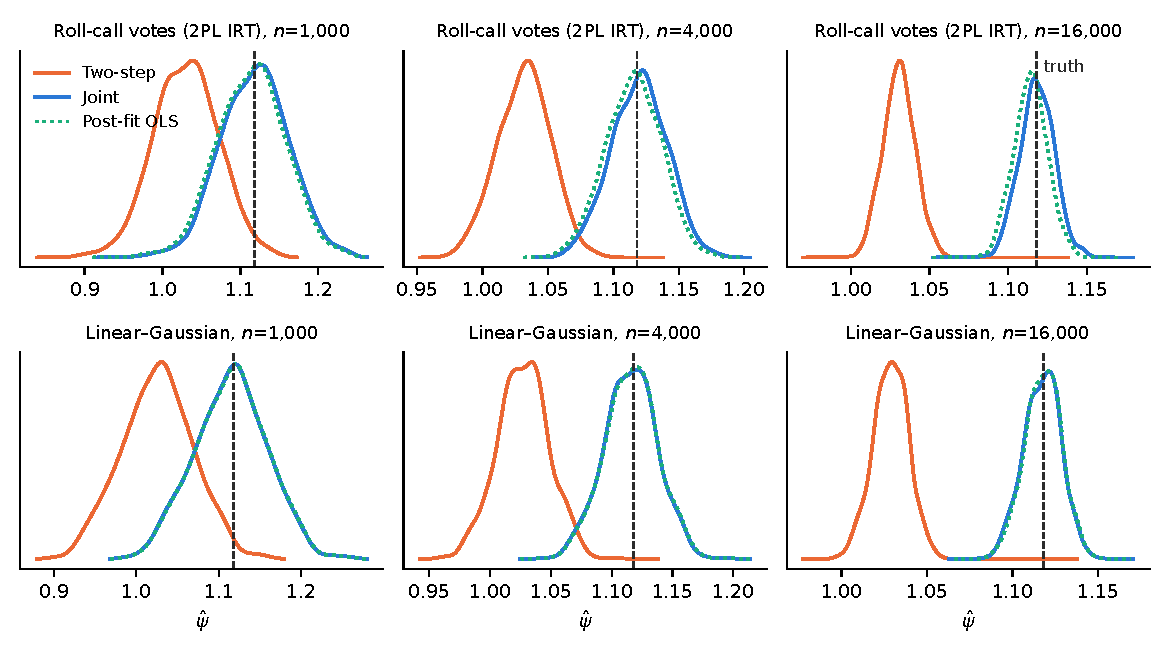
\includegraphics[width=\textwidth]{figures/sim_distributions.pdf}
\caption{Monte Carlo sampling distributions of $\hat\psi$ (kernel density
estimates over $1{,}000$ replications).  Rows: measurement channel;
columns: sample size.  Dashed line: truth $\psi=1.118$.  The two-step
distribution (orange) keeps its width but not its center as $n$ grows; the
joint estimator (blue) and its post-fit OLS readout (green, dotted)
concentrate on the truth.}
\label{fig:sim-distributions}
\end{figure}

\begin{figure}[t]
\centering
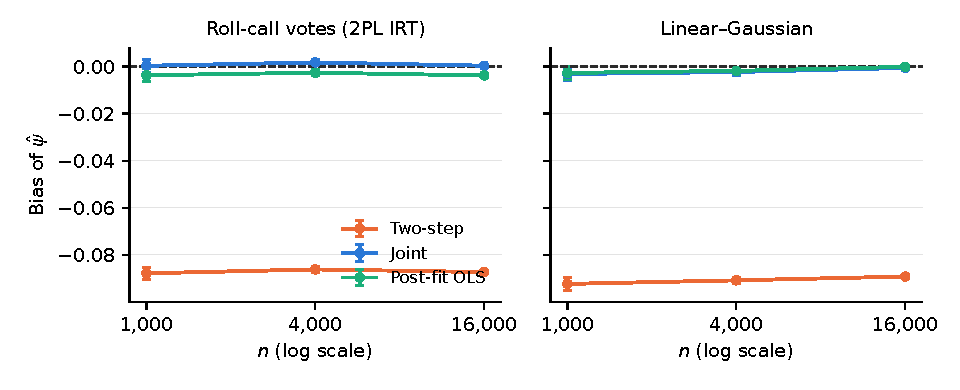
\includegraphics[width=\textwidth]{figures/sim_bias.pdf}
\caption{Bias of $\hat\psi$ against sample size (log scale); vertical bars
are $\pm2$ Monte Carlo standard errors.  The two-step bias is flat at
$-0.09$ while its sampling noise shrinks---the $\kappa>0$ signature; the
joint and post-fit estimators are unbiased at every $n$.}
\label{fig:sim-bias}
\end{figure}

\subsection{Inference: coverage collapse and a corrected interval}
\label{sec:sim-inference}

\begin{table}[t]
\centering
\caption{Empirical coverage of nominal 95\% confidence intervals for
$\psi$ (binomial standard errors in parentheses; $1{,}000$ replications per
cell).  Two-step: textbook OLS interval around the two-step estimate.
Post-fit naive: OLS interval around the post-fit estimate.  Post-fit
corrected: same center, standard error inflated by the delta-method term
in~\eqref{eq:sim-secorr}.}
\label{tab:sim-coverage}
\begin{tabular}{lccc}
\toprule
$n$ & Two-step (naive) & Post-fit (naive) & Post-fit (corrected) \\
\midrule
\multicolumn{4}{l}{\emph{Panel: Roll-call votes (2PL IRT)}} \\
1,000 & 0.307 (0.015) & 0.911 (0.009) & 0.956 (0.006) \\
4,000 & 0.004 (0.002) & 0.909 (0.009) & 0.960 (0.006) \\
16,000 & 0.000 (0.000) & 0.881 (0.010) & 0.940 (0.008) \\
\midrule
\multicolumn{4}{l}{\emph{Panel: Linear--Gaussian}} \\
1,000 & 0.284 (0.014) & 0.895 (0.010) & 0.960 (0.006) \\
4,000 & 0.002 (0.001) & 0.900 (0.009) & 0.953 (0.007) \\
16,000 & 0.000 (0.000) & 0.908 (0.009) & 0.962 (0.006) \\
\bottomrule
\end{tabular}

\end{table}

Table~\ref{tab:sim-coverage} and Figure~\ref{fig:sim-coverage} translate
the location shift into inference.  The naive two-step interval has
approximately the right width---its OLS standard error is close to the true
sampling standard deviation---but it is centered at the wrong point, so its
coverage is $0.31$ at $n=1{,}000$, $0.004$ at $n=4{,}000$, and $0.000$ at
$n=16{,}000$: at the largest sample size, not one interval in a thousand
contained the truth.  This is the practical content of the $\kappa>0$
asymptotics: the bias is fixed while the interval width shrinks like
$1/\sqrt{n}$, so the interval slides off the truth at rate $\sqrt{n}$, and
more data makes the inference more confidently wrong.

The post-fit OLS interval is correctly centered, and its naive version
already covers $0.88$--$0.93$.  The remaining shortfall has a transparent
source: the estimand $\psi=c\,\sigma_\theta$ is a product, and the OLS
standard error accounts only for the noise in the slope $\hat c$, not for
the noise in the scale $\hat\sigma_\theta$.  A delta-method argument gives
the missing term.  Since
$\mathrm{var}(\hat\sigma_\theta^2)\approx(\kappa_\theta-1)\,\sigma_\theta^4/n$
for a marginal with kurtosis $\kappa_\theta$,
\begin{equation}
  \widehat{\mathrm{SE}}_{\mathrm{corr}}^2(\hat\psi)
  \;=\;
  \widehat{\mathrm{SE}}_{\mathrm{OLS}}^2\cdot\hat\sigma_\theta^2
  \;+\;
  \hat\psi^{\,2}\,\frac{\hat\kappa_\theta-1}{4n},
  \label{eq:sim-secorr}
\end{equation}
where $\hat\kappa_\theta$ is the plug-in kurtosis of the model-implied
marginal of $\theta$ (available in closed form from the fitted prior; for
our two-component design its true value is $2.92$, below the Gaussian
$3$).  Everything in~\eqref{eq:sim-secorr} comes out of the fitted model
and the regression output---no resampling, no extra optimization.

The corrected interval covers between $0.940$ and $0.962$ in the six core
cells, pooling to $0.955$ across $6{,}000$ replications, against the
nominal $0.95$.  The correction matters more, not less, as measurement
improves: in the $J=100$ cell the slope is estimated very precisely, so the
neglected $\hat\sigma_\theta$ noise dominates and naive coverage falls to
$0.88$, while the corrected interval covers $0.95$
(Figure~\ref{fig:sim-mechanism}b).

\begin{figure}[t]
\centering
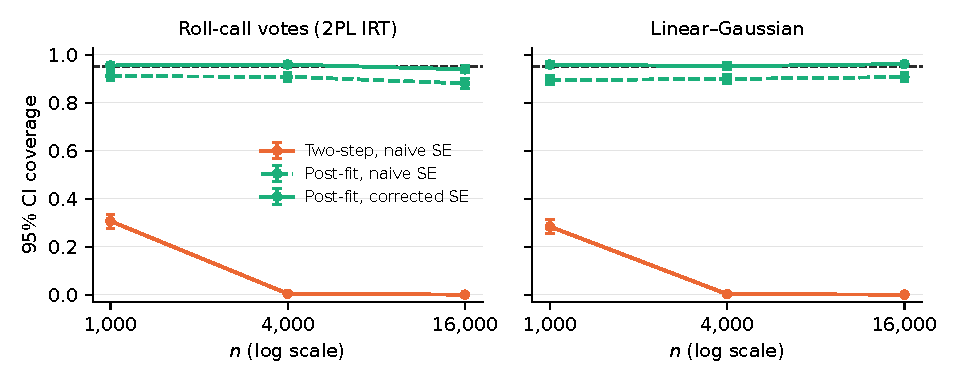
\includegraphics[width=\textwidth]{figures/sim_coverage.pdf}
\caption{Coverage of nominal 95\% intervals for $\psi$ by sample size.
The two-step interval collapses to zero coverage; the post-fit interval
with the corrected standard error~\eqref{eq:sim-secorr} attains nominal
coverage at every $n$ in both channels.}
\label{fig:sim-coverage}
\end{figure}

\subsection{The mechanism: reliability, not approximation error}
\label{sec:sim-mechanism}

\begin{figure}[t]
\centering
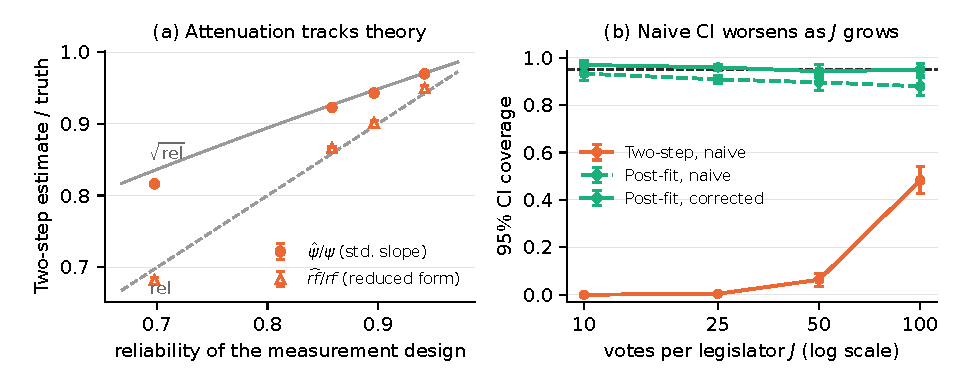
\includegraphics[width=\textwidth]{figures/sim_mechanism.pdf}
\caption{(a) Two-step attenuation against the reliability of the
measurement design, varied through $J\in\{10,25,50,100\}$ at $n=4{,}000$
(vote channel).  The standardized slope tracks $\sqrt{\mathrm{rel}}$ and
the reduced form tracks $\mathrm{rel}$, the errors-in-variables
predictions, with no free parameters.  (b) Coverage against $J$: more votes
shrink the two-step bias but its interval also shrinks, so coverage remains
far below nominal even at $J=100$; the corrected post-fit interval is
nominal throughout, while the \emph{naive} post-fit interval deteriorates
as $J$ grows.}
\label{fig:sim-mechanism}
\end{figure}

Figure~\ref{fig:sim-mechanism}(a) closes the loop between the measured
biases and the theory.  Varying the number of votes traces reliability from
$0.70$ ($J=10$) to $0.94$ ($J=100$), and the observed two-step attenuation
follows the errors-in-variables predictions essentially exactly: the
standardized slope attenuates by $\sqrt{\mathrm{rel}}$ (observed ratio to
truth $0.82/0.92/0.94/0.97$ against predicted $0.84/0.93/0.95/0.97$) and
the reduced form by $\mathrm{rel}$ itself.  Two further diagnostics pin
down that reliability is the \emph{only} active mechanism.  First, the
oracle benchmark: OLS of $y$ on the exact posterior mean under the true DGP
is per-unit unbiased ($\hat c$ between $0.999$ and $1.001$ in every cell),
so posterior-mean shrinkage per se does not bias the per-unit slope; the
two-step bias in $\psi$ arises from standardizing by the deflated scale of
the shrunken factor estimates, compounded by the misspecified fixed prior.
Second, variational inference is exonerated: the correlation between
estimated and true factors sits at its feasible ceiling
$\sqrt{\mathrm{rel}}$ (e.g.\ $0.922$ against a ceiling of $0.927$ in the
vote channel), mean-field credible intervals for $\theta_i$ attain $0.89$
average coverage against the exact posterior's $0.90$ at nominal $0.90$,
and the exact-posterior two-step arm reproduces the VI two-step arm's bias.
The two-step problem is econometric, not computational, and it cannot be
fixed by a better approximation to the unsupervised posterior---only by
changing the estimand of the first step, which is what joint estimation
does.  (Full VI diagnostics are reported in
Table~\ref{tab:sim-vi-appendix}.)

\subsection{Summary and recommended procedure}
\label{sec:sim-recipe}

The simulations confirm each element of the theoretical account at Monte
Carlo precision: a flat, reliability-determined two-step bias with coverage
collapsing at rate $\sqrt{n}$; a joint estimator that is unbiased,
$\sqrt{n}$-consistent, and Gaussian in both a nonlinear and an exactly
tractable channel; equality of the two sampling spreads (a pure location
shift); and validity of a simple corrected interval.  For applied work the
procedure is:
\begin{enumerate}
\item estimate the measurement model and the outcome equation jointly
  (the supervised ELBO);
\item read out outcome-free posterior means under the fitted measurement
  model and regress the outcome on them by OLS;
\item report the OLS point estimate with the standard error
  inflated as in~\eqref{eq:sim-secorr}.
\end{enumerate}
Each step uses standard tooling, adds negligible computation to the fit,
and---in $6{,}900$ replications across nine designs---delivers unbiased
point estimates and nominal 95\% coverage where the prevailing two-step
practice delivers a fixed bias and, at realistic sample sizes, coverage
of zero.

% ---------- appendix table (place in the appendix) ----------
\begin{table}[t]
\centering
\caption{Variational-inference diagnostics ($J=25$ cells).
$\mathrm{corr}(\hat\theta,\theta)$: correlation of two-step posterior means
with the true factors, against its feasible ceiling
$\sqrt{\mathrm{rel}}$.  $\theta$-coverage: average coverage of nominal
90\% credible intervals for $\theta_i$, mean-field VI versus the exact
posterior (Gauss--Hermite).  Last column: per-unit slope of OLS on the
exact posterior mean (regression-calibration benchmark; truth $1$).}
\label{tab:sim-vi-appendix}
\begin{tabular}{lccccc}
\toprule
$n$ & $\mathrm{corr}(\hat\theta,\theta)$ & $\sqrt{\mathrm{rel}}$ ceiling & $\theta$-cov.\ (VI) & $\theta$-cov.\ (exact) & Oracle-PM $\hat c$ (per unit) \\
\midrule
\multicolumn{6}{l}{\emph{Panel: Roll-call votes (2PL IRT)}} \\
1,000 & 0.922 & 0.926 & 0.885 & 0.902 & 1.001 \\
4,000 & 0.922 & 0.927 & 0.887 & 0.902 & 1.001 \\
16,000 & 0.922 & 0.927 & 0.889 & 0.902 & 1.000 \\
\midrule
\multicolumn{6}{l}{\emph{Panel: Linear--Gaussian}} \\
1,000 & 0.919 & 0.923 & 0.887 & 0.900 & 1.000 \\
4,000 & 0.919 & 0.924 & 0.888 & 0.900 & 0.999 \\
16,000 & 0.920 & 0.925 & 0.889 & 0.900 & 1.000 \\
\bottomrule
\end{tabular}

\end{table}
